\section{Resultados}
En la figura \ref{fig: phase plot x} 
se presenta el diagrama fase del sistema para
posición y velocidad con respecto al eje $x$.

\begin{figure}[hb]
 \centering 
 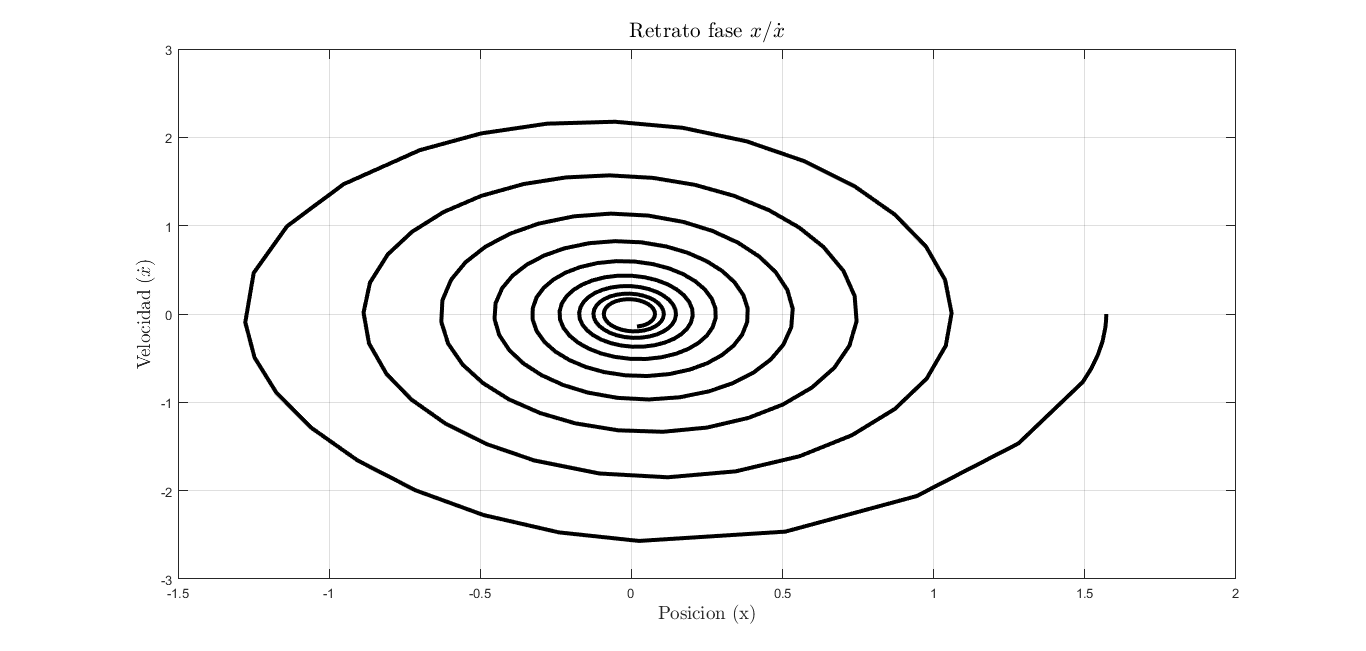
\includegraphics[scale=0.35]{./img/fasependulox2.png}
 % fasependulox2.png: 1853x1003 px, 96dpi, 49.02x26.53 cm, bb=0 0 1390 752
\caption{Diagrama de fase de $x(t)$ y $\dot{x}(t)$.}
 \label{fig: phase plot x}
\end{figure}



\begin{figure}[hb]
 \centering 
 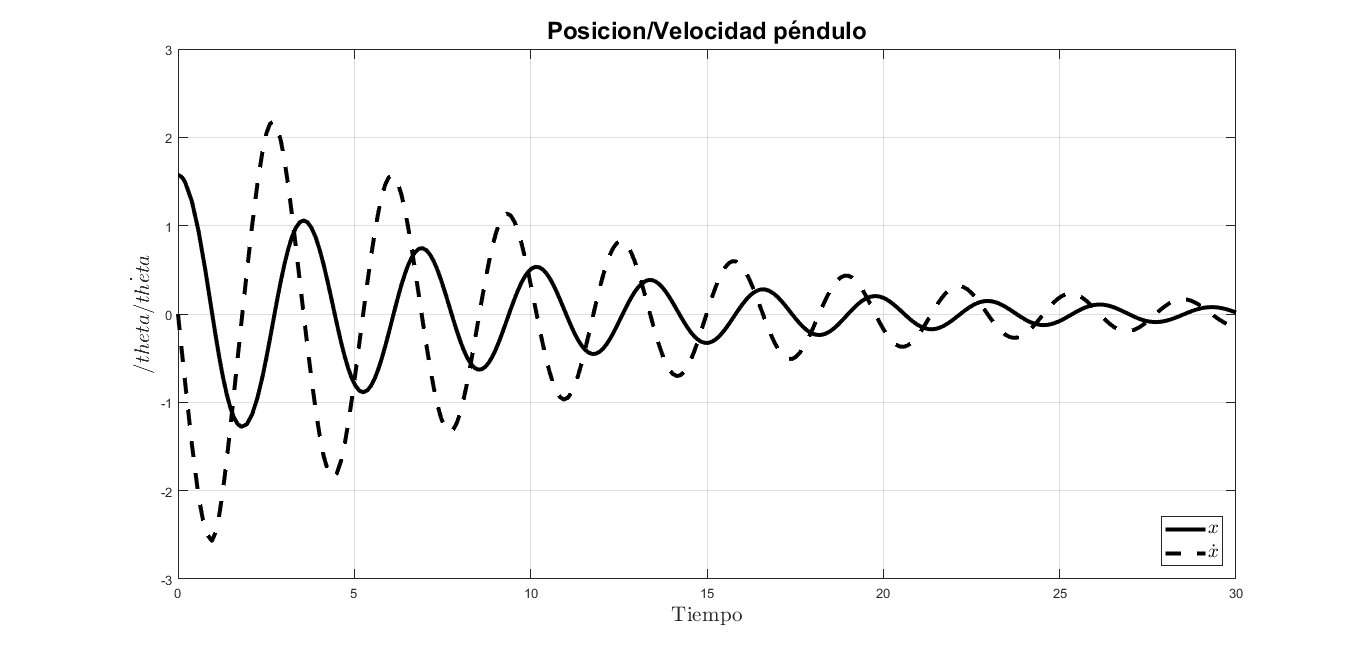
\includegraphics[scale=0.35]{./img/posvelpendulo2.png}
 % fasependulox2.png: 1853x1003 px, 96dpi, 49.02x26.53 cm, bb=0 0 1390 752
 \caption{Comportamiento de $x(t)$ y $\dot{x}(t)$ en el tiempo.}
 \label{fig: time plot x dx}
\end{figure}


\begin{figure}[h]
 \centering
 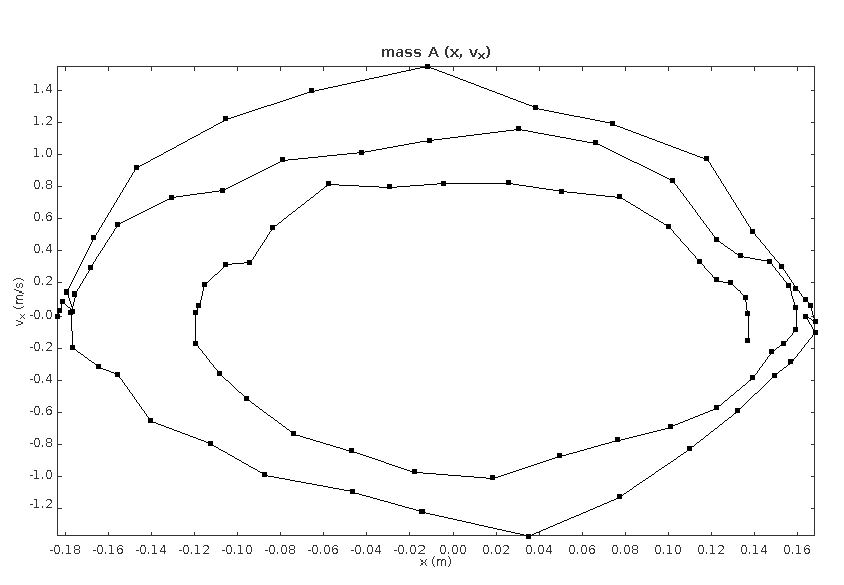
\includegraphics[scale=0.3]{./img/tracker_poc_phasediagram_x_vx.png}
 % tracker_poc_phasediagram_x_vx.png: 844x585 px, 72dpi, 29.78x20.64 cm, bb=0 0 844 585
 \caption{Diagrama de fase del modelo físico para $x$ y $\dot{x}$}
 \label{fig: tracker phase diagram x vx}
\end{figure}

\begin{figure}[h]
 \centering
 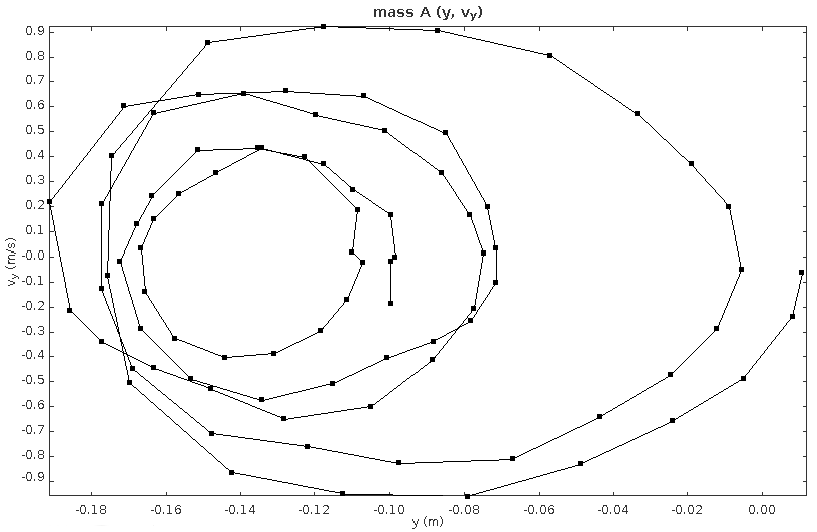
\includegraphics[scale=0.3]{./img/tracker_poc_phasediagram_y_vy.png}
 % tracker_poc_phasediagram_x_vx.png: 844x585 px, 72dpi, 29.78x20.64 cm, bb=0 0 844 585
 \caption{Diagrama de fase del modelo físico para $y$ y $\dot{y}$}
 \label{fig: tracker phase diagram y vy}
\end{figure}
